% !TEX program = latex
% 10 分钟短报告：10 页正文 + 1 页附录。搜索【并逐项替换。
\documentclass[aspectratio=169,11pt,fontset=fandol]{ctexbeamer}
\usepackage{ctextalk}

\title{【研究问题式标题】}
\subtitle{【研究对象与方法定位】}
\author{【姓名 · 单位 / 研究组】}
\date{【汇报日期】}

\begin{document}

% 01 封面。
\coverslide{【一行样本规模或方法定位】}
\note{直接提出研究问题，不念标题。}

% 02 两问目录。
\agendatwo{【研究问题一】}{【研究问题二】}

% 03 任务与样本：只保留理解结果所需的一条任务链。
\begin{frame}{【任务与分析样本如何对应】}
  \begin{columns}[T,onlytextwidth]
    \column{.43\textwidth}
      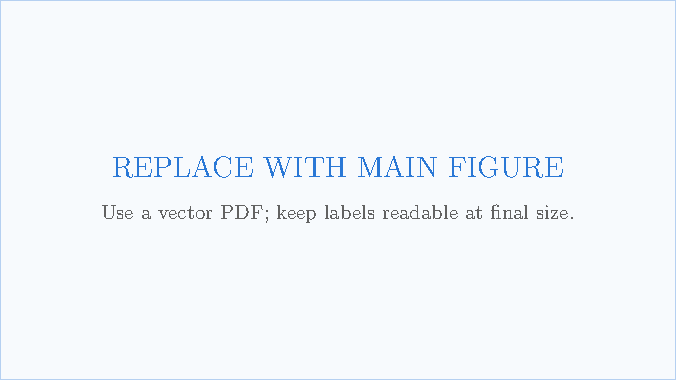
\includegraphics[width=\linewidth,height=.48\textheight,keepaspectratio]{figures/placeholder.pdf}\par
      \visualnote{【图中对象、条件和来源。】}
    \column{.52\textwidth}
      {\color{Accent}参与者完成什么}\par
      \fillin{任务目标与一次真实行为。}\par
      \vspace{.8em}
      {\color{Accent}哪些记录进入分析}\par
      \fillin{纳入条件、分析单位与最终样本量。}\par
      \vspace{.8em}
      {\color{Accent}哪些信息由原始记录重建}\par
      \fillin{只写理解模型所需的缺失信息或预处理。}
  \end{columns}
  \source{【刺激、数据版本与样本来源。】}
\end{frame}

% 04 分析流程。
\begin{frame}{【分析如何把行为转成研究证据】}
  \vspace{1.2em}
  \begin{columns}[c,onlytextwidth]
    \column{.27\textwidth}
      \centering\flowbox{输入}{\fillin{行为记录}\par\vspace{.3em}\fillin{已知条件}}
    \column{.06\textwidth}\centering{\color{Accent}\Large $\rightarrow$}
    \column{.36\textwidth}
      \centering\flowbox{模型}{\fillin{核心变量}\par\vspace{.3em}{\small\fillin{控制与验证}}}
    \column{.06\textwidth}\centering{\color{Accent}\Large $\rightarrow$}
    \column{.23\textwidth}
      \centering\flowbox{输出}{\fillin{估计或预测}}
  \end{columns}
  \takeaway{【模型比较的对象与输出。】}
\end{frame}

% 05 模型：只保留理解结果所需的一个公式。
\begin{frame}{【模型如何评价新增信息】}
  \centering
  \fcolorbox{Accent!25}{Accent!5}{%
    \begin{minipage}[c][2.2cm][c]{.82\linewidth}
      \centering{\Large $\displaystyle \text{【核心模型或评价公式】}$}
    \end{minipage}}\par
  \vspace{.8em}
  \begin{columns}[T,onlytextwidth]
    \column{.47\textwidth}
      {\color{Accent}基线与对照}\par
      \fillin{已有信息、核心变量和新增项。}
    \column{.47\textwidth}
      {\color{Accent}验证与不确定性}\par
      \fillin{样本划分单位、评价指标与区间类型。}
  \end{columns}
  \takeaway{【如何区分新增信息与已有解释。】}
\end{frame}

% 06–07 两页结果严格对应第 2 页。
\fullfigureslide
  {【结果一：回答研究问题一】}
  {figures/placeholder.pdf}
  {【横轴含义与单位】}
  {【纵轴含义与单位】}
  {【点、线、误差带与颜色含义】}
  {【结果一的 take-home message】}
  {【模型、样本、区间与数据来源】}

\fullfigureslide
  {【结果二：回答研究问题二】}
  {figures/placeholder.pdf}
  {【横轴含义与单位】}
  {【纵轴含义与单位】}
  {【点、线、误差带与颜色含义】}
  {【结果二的 take-home message】}
  {【模型、样本、区间与数据来源】}

% 08 边界：只保留会改变结论含义的限制。
\threepointslide{【结论能够推广到哪里】}
  {【样本边界】}{【目标总体与纳入范围。】}
  {【测量边界】}{【代理变量不能代表什么。】}
  {【推断边界】}{【相关、因果与外部效度限制。】}

% 09 结论：逐一回答两问，不引入新结果。
\twopointslide{【一句话概括整项研究】}
  {【回答问题一】}{【对应结果一的意义。】}
  {【回答问题二】}{【对应结果二的意义。】}

% 10 结束页。
\closingslide{谢谢，欢迎讨论}{【一句话核心结论】}

\appendix

% 11 附录核查：短报告仍保留必要的可复核性。
\begin{frame}{附录：【数值与实现核查的覆盖范围】}
  \setlength{\tabcolsep}{3pt}
  \begin{tabular}{@{}p{3.0cm} p{6.0cm} p{4.5cm}@{}}
    \toprule
    核查对象 & 方法与独立对照 & 覆盖范围 / 结果 \\
    \midrule
    【样本一致性】 & 【独立重算或跨表核对】 & 【数量与版本】 \\
    【实现正确性】 & 【解析解、测试或独立实现】 & 【最大差值】 \\
    【不确定性】 & 【重抽样或敏感性分析】 & 【覆盖范围与限制】 \\
    \bottomrule
  \end{tabular}
  \source{【代码、数据版本与冻结结果来源。】}
\end{frame}

\end{document}
